%===================================================================================================
% Beamer presentation generated from the notebook: chapter-08-01.ipynb
% Topic: Pre-trained Language Models, BERT, DistilBERT, and Text Classification
%===================================================================================================

\documentclass[aspectratio=169]{beamer}

%===================================================================================================
% Theme and packages
%===================================================================================================

\usetheme{Madrid}
\usecolortheme{default}

\usepackage[utf8]{inputenc}
\usepackage[T1]{fontenc}
\usepackage{lmodern}
\usepackage{amsmath, amssymb}
\usepackage{booktabs}
\usepackage{graphicx}
\usepackage{xcolor}
\usepackage{listings}
\usepackage{tikz}
\usetikzlibrary{positioning, arrows.meta, shapes.geometric}

%===================================================================================================
% Colors and listings
%===================================================================================================

\definecolor{codegray}{RGB}{245,245,245}
\definecolor{codeblue}{RGB}{34,80,150}
\definecolor{darkgreen}{RGB}{0,115,60}

\lstdefinestyle{pythonstyle}{
    language=Python,
    basicstyle=\ttfamily\scriptsize,
    keywordstyle=\color{codeblue}\bfseries,
    commentstyle=\color{darkgreen},
    stringstyle=\color{purple},
    backgroundcolor=\color{codegray},
    showstringspaces=false,
    breaklines=true,
    frame=single,
    rulecolor=\color{black!20},
    tabsize=4
}

\setbeamertemplate{navigation symbols}{}
\setbeamertemplate{footline}[frame number]

%===================================================================================================
% Title information
%===================================================================================================

\title[]{Chapter 5 Lab -- Pre-trained Language Models, BERT, DistilBERT, and Text Classification}
\subtitle{Advanced Machine Learning for Finance}
\author{Giovanni Della Lunga}
\institute{Master's Degree in Quantitative Finance -- University of Bologna}
\date{Bologna -- 2026}
%
%===================================================================================================
%

%===================================================================================================
\begin{document}
%===================================================================================================

\begin{frame}
    \titlepage
\end{frame}

%---------------------------------------------------------------------------------------------------
\begin{frame}{Learning objectives}
At the end of this notebook, students should be able to:
\begin{itemize}
    \item explain the idea of pre-trained language models and transfer learning;
    \item understand why BERT is an encoder-based Transformer model for language understanding;
    \item use Hugging Face tokenizers to prepare text inputs for BERT-like models;
    \item run sentiment inference with a pre-trained DistilBERT classifier;
    \item build a PyTorch dataset, classifier, training loop, and evaluation function for news classification.
\end{itemize}
\end{frame}

%---------------------------------------------------------------------------------------------------
\begin{frame}{Notebook structure}
The notebook develops the topic in two main parts.

\vspace{0.3cm}

\begin{columns}
\column{0.48\textwidth}
\textbf{Part 1: using pre-trained models}
\begin{itemize}
    \item pre-trained language models;
    \item transfer learning;
    \item BERT and tokenization;
    \item DistilBERT sentiment analysis;
    \item Hugging Face \texttt{pipeline}.
\end{itemize}

\column{0.48\textwidth}
\textbf{Part 2: fine-tuning for classification}
\begin{itemize}
    \item BBC News dataset;
    \item text preprocessing;
    \item PyTorch \texttt{Dataset} and \texttt{DataLoader};
    \item custom BERT classifier;
    \item training, validation, and test evaluation.
\end{itemize}
\end{columns}
\end{frame}

%---------------------------------------------------------------------------------------------------
\begin{frame}{What is a pre-trained language model?}
A pre-trained language model is a neural network first trained on a very large text corpus, before being adapted to a specific downstream task.

\vspace{0.3cm}

The main idea is that the model learns general linguistic regularities:
\begin{itemize}
    \item syntactic patterns;
    \item semantic relations;
    \item contextual word usage;
    \item statistical regularities of natural language.
\end{itemize}

\vspace{0.2cm}

Once learned, these representations can be reused for tasks such as sentiment analysis, named entity recognition, text classification, question answering, and summarization.
\end{frame}

%---------------------------------------------------------------------------------------------------
\begin{frame}{Why pre-training matters}
Training a modern language model from scratch is expensive because it requires:
\begin{itemize}
    \item a very large corpus;
    \item substantial computational resources;
    \item long training time;
    \item careful optimization and engineering.
\end{itemize}

\vspace{0.3cm}

Using a pre-trained model allows us to start from a network that already contains a rich representation of language. The downstream model does not learn language from zero; it learns how to use linguistic representations for a specific task.
\end{frame}

%---------------------------------------------------------------------------------------------------
\begin{frame}{Transfer learning in NLP}
Transfer learning means that knowledge acquired while solving one task is reused for another related task.

\vspace{0.3cm}

In NLP, the usual workflow is:
\begin{enumerate}
    \item \textbf{Pre-training}: train a large model on a broad language objective.
    \item \textbf{Feature extraction}: use the model to produce contextual embeddings.
    \item \textbf{Fine-tuning}: add a task-specific head and train on the target dataset.
\end{enumerate}

\vspace{0.3cm}

Fine-tuning may update all model parameters, or only the parameters of the task-specific layers.
\end{frame}

%---------------------------------------------------------------------------------------------------
\begin{frame}{Freezing versus fine-tuning}
\begin{columns}
\column{0.48\textwidth}
\textbf{Frozen encoder}
\begin{itemize}
    \item BERT weights are kept fixed.
    \item Only the classification head is trained.
    \item Training is faster and cheaper.
    \item Useful when little data is available.
\end{itemize}

\column{0.48\textwidth}
\textbf{Full fine-tuning}
\begin{itemize}
    \item Both BERT and the classification head are updated.
    \item The model adapts more deeply to the target task.
    \item Usually gives better performance.
    \item Requires more care to avoid overfitting.
\end{itemize}
\end{columns}
\end{frame}

%---------------------------------------------------------------------------------------------------
\begin{frame}{BERT: Bidirectional Encoder Representations from Transformers}
BERT is an encoder-based Transformer architecture introduced for language understanding tasks.

\vspace{0.3cm}

Its key feature is \textbf{bidirectionality}: each token representation is computed using both left and right context.

\vspace{0.3cm}

For example, in the sentence:
\begin{center}
\textit{The bank approved the loan.}
\end{center}

the representation of the word \textit{bank} depends on the surrounding words \textit{approved} and \textit{loan}, not only on the words before it.
\end{frame}

%---------------------------------------------------------------------------------------------------
\begin{frame}{BERT architecture at a high level}
\begin{center}
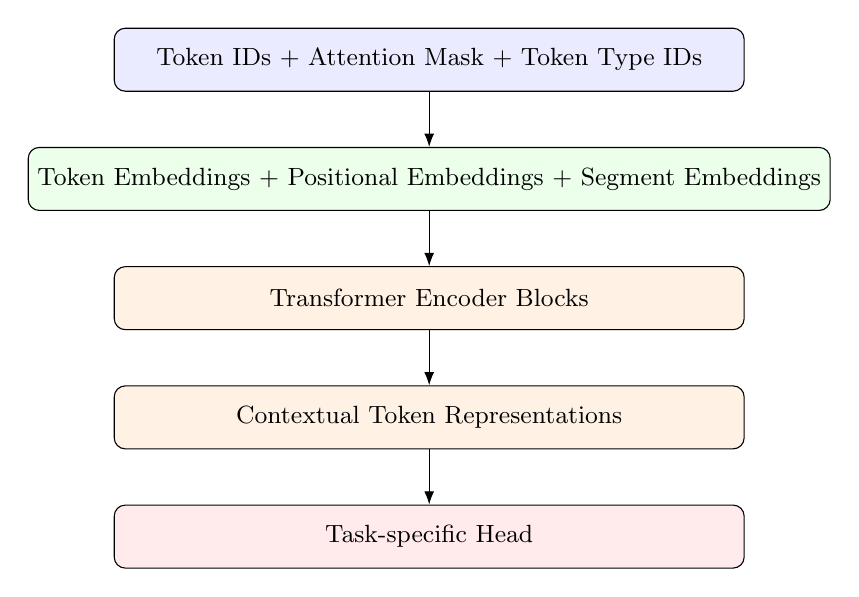
\begin{tikzpicture}[node distance=0.7cm, every node/.style={font=\small}]
    \node[draw, rounded corners, fill=blue!8, minimum width=8cm, minimum height=0.8cm] (input) {Token IDs + Attention Mask + Token Type IDs};
    \node[draw, rounded corners, fill=green!8, minimum width=8cm, minimum height=0.8cm, below=of input] (emb) {Token Embeddings + Positional Embeddings + Segment Embeddings};
    \node[draw, rounded corners, fill=orange!10, minimum width=8cm, minimum height=0.8cm, below=of emb] (enc1) {Transformer Encoder Blocks};
    \node[draw, rounded corners, fill=orange!10, minimum width=8cm, minimum height=0.8cm, below=of enc1] (enc2) {Contextual Token Representations};
    \node[draw, rounded corners, fill=red!8, minimum width=8cm, minimum height=0.8cm, below=of enc2] (head) {Task-specific Head};
    \draw[-{Latex}] (input) -- (emb);
    \draw[-{Latex}] (emb) -- (enc1);
    \draw[-{Latex}] (enc1) -- (enc2);
    \draw[-{Latex}] (enc2) -- (head);
\end{tikzpicture}
\end{center}
\end{frame}

%---------------------------------------------------------------------------------------------------
\begin{frame}{BERT base and BERT large}
\begin{center}
\begin{tabular}{lccc}
\toprule
\textbf{Model} & \textbf{Encoder layers} & \textbf{Attention heads} & \textbf{Hidden size} \\
\midrule
BERT base & 12 & 12 & 768 \\
BERT large & 24 & 16 & 1024 \\
\bottomrule
\end{tabular}
\end{center}

\vspace{0.4cm}

The notebook uses BERT mainly as a conceptual foundation, then moves to DistilBERT for a sentiment analysis example and to \texttt{bert-base-cased} for the custom news classifier.
\end{frame}

%---------------------------------------------------------------------------------------------------
\begin{frame}[fragile]{First tokenization example}
The notebook starts by using the Hugging Face BERT tokenizer.

\begin{lstlisting}[style=pythonstyle]
from transformers import BertTokenizer

tokenizer = BertTokenizer.from_pretrained('bert-base-uncased')
text = "BERT preprocessing is essential."
tokens = tokenizer.tokenize(text)

print(tokens)
\end{lstlisting}

\vspace{0.2cm}

The tokenizer converts raw text into subword tokens that can be mapped into integer IDs and passed to the model.
\end{frame}

%---------------------------------------------------------------------------------------------------
\begin{frame}{What the tokenizer produces}
A BERT tokenizer usually returns a dictionary containing several tensors.

\vspace{0.3cm}

\begin{center}
\begin{tabular}{ll}
\toprule
\textbf{Key} & \textbf{Meaning} \\
\midrule
\texttt{input\_ids} & Integer IDs representing tokens. \\
\texttt{attention\_mask} & Indicates real tokens versus padding tokens. \\
\texttt{token\_type\_ids} & Indicates sentence A versus sentence B when needed. \\
\bottomrule
\end{tabular}
\end{center}

\vspace{0.3cm}

These tensors are the actual numerical input consumed by BERT-like models.
\end{frame}

%---------------------------------------------------------------------------------------------------
\begin{frame}{Special tokens}
BERT adds special tokens to the original text.

\vspace{0.3cm}

\begin{itemize}
    \item \texttt{[CLS]}: placed at the beginning of the sequence. Its final representation is often used for classification.
    \item \texttt{[SEP]}: marks the end of a sequence, or separates two sequences.
    \item \texttt{[PAD]}: fills shorter sequences so that all examples in a batch have the same length.
\end{itemize}

\vspace{0.3cm}

For a single-sequence classification task, the model can use the contextual representation of \texttt{[CLS]} as a compact summary of the whole input sentence.
\end{frame}

%---------------------------------------------------------------------------------------------------
\begin{frame}{Attention mask}
The attention mask tells the model which tokens should be considered.

\vspace{0.3cm}

\begin{center}
\begin{tabular}{ccc}
\toprule
\textbf{Token} & \textbf{Example ID} & \textbf{Attention mask} \\
\midrule
\texttt{[CLS]} & 101 & 1 \\
\texttt{bert} & 14324 & 1 \\
\texttt{preprocessing} & 17463 & 1 \\
\texttt{[SEP]} & 102 & 1 \\
\texttt{[PAD]} & 0 & 0 \\
\bottomrule
\end{tabular}
\end{center}

\vspace{0.3cm}

A value of 1 means that the token is meaningful; a value of 0 means that the token is padding and should be ignored by attention.
\end{frame}

%---------------------------------------------------------------------------------------------------
\begin{frame}{Distilled models}
A distilled language model is a smaller model trained to imitate a larger teacher model.

\vspace{0.3cm}

\begin{center}
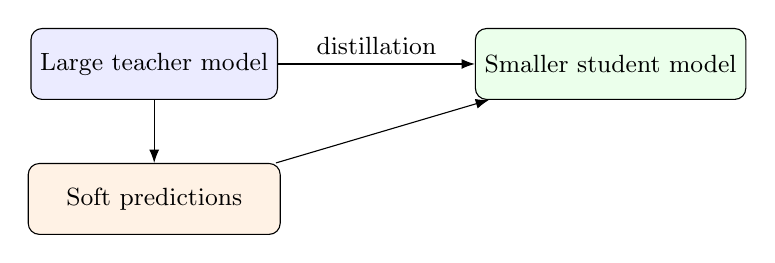
\begin{tikzpicture}[node distance=1cm, every node/.style={font=\small}]
    \node[draw, rounded corners, fill=blue!8, minimum width=3cm, minimum height=0.9cm] (teacher) {Large teacher model};
    \node[draw, rounded corners, fill=green!8, minimum width=3cm, minimum height=0.9cm, right=2.5cm of teacher] (student) {Smaller student model};
    \node[draw, rounded corners, fill=orange!10, minimum width=3.2cm, minimum height=0.9cm, below=0.8cm of teacher] (knowledge) {Soft predictions};
    \draw[-{Latex}] (teacher) -- node[above]{distillation} (student);
    \draw[-{Latex}] (teacher) -- (knowledge);
    \draw[-{Latex}] (knowledge) -- (student);
\end{tikzpicture}
\end{center}

\vspace{0.2cm}

DistilBERT is designed to retain much of BERT's performance while reducing model size and inference cost.
\end{frame}

%---------------------------------------------------------------------------------------------------
\begin{frame}[fragile]{Loading a pre-trained DistilBERT sentiment model}
The notebook loads a DistilBERT model already fine-tuned on a binary sentiment classification task.

\begin{lstlisting}[style=pythonstyle]
from transformers import DistilBertTokenizer, DistilBertForSequenceClassification
import torch

tokenizer = DistilBertTokenizer.from_pretrained(
    'distilbert-base-uncased-finetuned-sst-2-english'
)

model = DistilBertForSequenceClassification.from_pretrained(
    'distilbert-base-uncased-finetuned-sst-2-english'
)
\end{lstlisting}

\vspace{0.2cm}

Here the model already contains both a language encoder and a sentiment classification head.
\end{frame}

%---------------------------------------------------------------------------------------------------
\begin{frame}[fragile]{Tokenizing two sentences}
The notebook then prepares two example sentences.

\begin{lstlisting}[style=pythonstyle]
sentence_a = 'i love this product, it helped me alot'
sentence_b = 'this does not work for me'

inputs = tokenizer(
    [sentence_a, sentence_b],
    return_tensors='pt',
    padding=True
)
\end{lstlisting}

\vspace{0.2cm}

The argument \texttt{return\_tensors='pt'} tells the tokenizer to return PyTorch tensors.
\end{frame}

%---------------------------------------------------------------------------------------------------
\begin{frame}[fragile]{From logits to predicted class}
The model produces logits, which are raw class scores before normalization.

\begin{lstlisting}[style=pythonstyle]
outputs = model(**inputs)
predicted_classes = torch.argmax(outputs.logits, dim=1)
\end{lstlisting}

\vspace{0.3cm}

Let $z_{i,k}$ be the logit for example $i$ and class $k$. The predicted class is:
\[
\hat{y}_i = \arg\max_k z_{i,k}
\]
where $\hat{y}_i$ is the predicted label for example $i$, and $z_{i,k}$ is the unnormalized model score for class $k$.
\end{frame}

%---------------------------------------------------------------------------------------------------
\begin{frame}[fragile]{Single-sentence prediction}
For one sentence, the notebook extracts the predicted class and maps it to a human-readable label.

\begin{lstlisting}[style=pythonstyle]
inputs = tokenizer(sentence_a, return_tensors='pt', padding=True)
outputs = model(**inputs)

predicted_class = torch.argmax(outputs.logits, dim=1).item()
class_labels = ['Negative', 'Positive']

print(f"The sentiment of the text is: {class_labels[predicted_class]}")
\end{lstlisting}
\end{frame}

%---------------------------------------------------------------------------------------------------
\begin{frame}[fragile]{Using the Hugging Face pipeline}
The notebook also shows the high-level \texttt{pipeline} interface.

\begin{lstlisting}[style=pythonstyle]
from transformers import pipeline

sentiment = pipeline(
    task='sentiment-analysis',
    framework='pt',
    model='distilbert-base-uncased-finetuned-sst-2-english'
)

results = sentiment('i am in a very bad mood today')
\end{lstlisting}

\vspace{0.2cm}

The pipeline hides tokenization, model inference, logits processing, and label decoding behind a compact API.
\end{frame}

%---------------------------------------------------------------------------------------------------
\begin{frame}{From simple inference to custom fine-tuning}
The second part of the notebook moves from using an already fine-tuned model to building a custom classifier.

\vspace{0.3cm}

The target task is BBC news classification into five categories:
\begin{center}
\texttt{business}, \texttt{entertainment}, \texttt{sport}, \texttt{tech}, \texttt{politics}
\end{center}

\vspace{0.3cm}

The goal is no longer to classify sentiment, but to assign each article to its correct news category.
\end{frame}

%---------------------------------------------------------------------------------------------------
\begin{frame}[fragile]{Loading the BBC News dataset}
The notebook expects a CSV file with two columns: category and text.

\begin{lstlisting}[style=pythonstyle]
import pandas as pd

datapath = './data/bbc-text.csv'
df = pd.read_csv(datapath)
df.head()
\end{lstlisting}

\vspace{0.2cm}

The category column contains the target label, while the text column contains the input article.
\end{frame}

%---------------------------------------------------------------------------------------------------
\begin{frame}[fragile]{Inspecting class frequencies}
Before training, the notebook checks the distribution of classes.

\begin{lstlisting}[style=pythonstyle]
df.groupby(['category']).size().plot.bar()
\end{lstlisting}

\vspace{0.3cm}

This is an important diagnostic step. If one class is much more frequent than the others, accuracy alone may become misleading.
\end{frame}

%---------------------------------------------------------------------------------------------------
\begin{frame}[fragile]{Tokenizing longer texts}
For the news classification task, the notebook uses \texttt{bert-base-cased}.

\begin{lstlisting}[style=pythonstyle]
tokenizer = BertTokenizer.from_pretrained('bert-base-cased')

bert_input = tokenizer(
    example_text,
    padding='max_length',
    max_length=60,
    truncation=True,
    return_tensors='pt'
)
\end{lstlisting}

\vspace{0.2cm}

The tokenizer automatically adds special tokens, pads shorter examples, and truncates longer examples.
\end{frame}

%---------------------------------------------------------------------------------------------------
\begin{frame}{The role of \texttt{[CLS]} in classification}
For a classification task, the notebook focuses on the pooled representation associated with \texttt{[CLS]}.

\vspace{0.3cm}

The intuition is:
\begin{itemize}
    \item BERT produces a contextual vector for each token;
    \item the final \texttt{[CLS]} representation is used as a sequence-level representation;
    \item the classifier maps this vector into category scores.
\end{itemize}

\vspace{0.3cm}

If $h_{\texttt{CLS}} \in \mathbb{R}^{768}$ is the BERT vector for \texttt{[CLS]}, the classification head transforms it into a vector of class scores.
\end{frame}

%---------------------------------------------------------------------------------------------------
\begin{frame}[fragile]{Label encoding}
Text labels are mapped into integers.

\begin{lstlisting}[style=pythonstyle]
labels = {
    'business'     : 0,
    'entertainment': 1,
    'sport'        : 2,
    'tech'         : 3,
    'politics'     : 4
}
\end{lstlisting}

\vspace{0.2cm}

Neural networks do not train directly on string labels. The target category must be represented numerically.
\end{frame}

%---------------------------------------------------------------------------------------------------
\begin{frame}{PyTorch Dataset and DataLoader}
The notebook introduces two fundamental PyTorch abstractions.

\vspace{0.2cm}

\begin{center}
\begin{tabular}{ll}
\toprule
\textbf{Object} & \textbf{Role} \\
\midrule
\texttt{Dataset} & Stores samples and labels; defines how to retrieve one item. \\
\texttt{DataLoader} & Creates mini-batches, shuffles data, and iterates during training. \\
\bottomrule
\end{tabular}
\end{center}

\vspace{0.3cm}

This separation keeps preprocessing and model training modular.
\end{frame}

%---------------------------------------------------------------------------------------------------
\begin{frame}[fragile]{Custom Dataset class}
The custom dataset tokenizes every article and stores the corresponding label.

\begin{lstlisting}[style=pythonstyle]
class Dataset(torch.utils.data.Dataset):
    def __init__(self, df):
        self.labels = [labels[label] for label in df['category']]
        self.texts = [tokenizer(text,
                                padding='max_length',
                                max_length=512,
                                truncation=True,
                                return_tensors="pt")
                      for text in df['text']]

    def __len__(self):
        return len(self.labels)

    def __getitem__(self, idx):
        return self.texts[idx], np.array(self.labels[idx])
\end{lstlisting}
\end{frame}

%---------------------------------------------------------------------------------------------------
\begin{frame}[fragile]{Train, validation, and test split}
The dataset is randomly shuffled and split into three subsets.

\begin{lstlisting}[style=pythonstyle]
np.random.seed(112)

df_train, df_val, df_test = np.split(
    df.sample(frac=1, random_state=42),
    [int(.8 * len(df)), int(.9 * len(df))]
)
\end{lstlisting}

\vspace{0.2cm}

The proportions are approximately:
\begin{center}
80\% training, 10\% validation, 10\% test.
\end{center}
\end{frame}

%---------------------------------------------------------------------------------------------------
\begin{frame}{The custom BERT classifier}
The notebook defines a class \texttt{BertClassifier} that inherits from \texttt{nn.Module}.

\vspace{0.2cm}

The model contains:
\begin{itemize}
    \item a pre-trained \texttt{BertModel};
    \item a dropout layer for regularization;
    \item a linear layer mapping a 768-dimensional BERT vector to 5 class scores;
    \item a ReLU activation in the notebook implementation.
\end{itemize}

\vspace{0.2cm}

The 768-dimensional input corresponds to the hidden size of BERT base.
\end{frame}

%---------------------------------------------------------------------------------------------------
\begin{frame}[fragile]{Classifier definition}
\begin{lstlisting}[style=pythonstyle]
from torch import nn
from transformers import BertModel

class BertClassifier(nn.Module):
    def __init__(self, dropout=0.5):
        super(BertClassifier, self).__init__()
        self.bert = BertModel.from_pretrained('bert-base-cased')
        self.dropout = nn.Dropout(dropout)
        self.linear = nn.Linear(768, 5)
        self.relu = nn.ReLU()
\end{lstlisting}

\vspace{0.2cm}

The final output has dimension 5 because the BBC dataset has five classes.
\end{frame}

%---------------------------------------------------------------------------------------------------
\begin{frame}[fragile]{Forward pass}
The forward pass extracts the pooled \texttt{[CLS]} representation and feeds it to the classifier head.

\begin{lstlisting}[style=pythonstyle]
def forward(self, input_id, mask):
    _, pooled_output = self.bert(
        input_ids=input_id,
        attention_mask=mask,
        return_dict=False
    )

    dropout_output = self.dropout(pooled_output)
    linear_output = self.linear(dropout_output)
    final_layer = self.relu(linear_output)

    return final_layer
\end{lstlisting}
\end{frame}

%---------------------------------------------------------------------------------------------------
\begin{frame}{Forward pass as a mathematical map}
The classifier can be summarized as:
\[
h_{\texttt{CLS}} = \mathrm{BERT}(x, m)
\]
\[
z = W h_{\texttt{CLS}} + b
\]
\[
\hat{y} = \arg\max_k z_k
\]

where:
\begin{itemize}
    \item $x$ is the vector of input token IDs;
    \item $m$ is the attention mask;
    \item $h_{\texttt{CLS}}$ is the pooled BERT representation;
    \item $W$ and $b$ are the classifier weights and bias;
    \item $z_k$ is the score for class $k$;
    \item $\hat{y}$ is the predicted class.
\end{itemize}
\end{frame}

%---------------------------------------------------------------------------------------------------
\begin{frame}{Training objective}
The notebook uses cross-entropy loss for multi-class classification.

\[
\mathcal{L} = - \sum_{k=1}^{K} y_k \log p_k
\]

where:
\begin{itemize}
    \item $K=5$ is the number of news categories;
    \item $y_k$ is 1 if the true class is $k$ and 0 otherwise;
    \item $p_k$ is the predicted probability for class $k$;
    \item $\mathcal{L}$ is the loss minimized during training.
\end{itemize}

\vspace{0.2cm}

In PyTorch, \texttt{nn.CrossEntropyLoss()} expects raw logits as input and internally applies the softmax operation.
\end{frame}

%---------------------------------------------------------------------------------------------------
\begin{frame}[fragile]{Training setup}
The training function creates datasets, data loaders, loss function, optimizer, and device configuration.

\begin{lstlisting}[style=pythonstyle]
train, val = Dataset(train_data), Dataset(val_data)

train_dataloader = torch.utils.data.DataLoader(
    train, batch_size=2, shuffle=True
)
val_dataloader = torch.utils.data.DataLoader(
    val, batch_size=2
)

criterion = nn.CrossEntropyLoss()
optimizer = Adam(model.parameters(), lr=learning_rate)
\end{lstlisting}
\end{frame}

%---------------------------------------------------------------------------------------------------
\begin{frame}{Why \texttt{zero\_grad()} is needed}
PyTorch accumulates gradients by default.

\vspace{0.3cm}

Therefore, before computing a new gradient on a new mini-batch, we must clear the old gradients:
\[
\nabla_{\theta} \mathcal{L}_{\text{new batch}}
\]
should not be accidentally added to previous gradients.

\vspace{0.3cm}

In the training loop this is done by:
\begin{center}
\texttt{model.zero\_grad()}
\end{center}
where $\theta$ denotes all trainable model parameters.
\end{frame}

%---------------------------------------------------------------------------------------------------
\begin{frame}{Training loop logic}
For each epoch, the notebook performs:
\begin{enumerate}
    \item iterate over mini-batches from the training set;
    \item move inputs and labels to CPU or GPU;
    \item compute model outputs;
    \item compute cross-entropy loss;
    \item compute gradients with backpropagation;
    \item update parameters with Adam;
    \item measure training accuracy and validation accuracy.
\end{enumerate}

\vspace{0.2cm}

The validation set is used to monitor generalization during training.
\end{frame}

%---------------------------------------------------------------------------------------------------
\begin{frame}[fragile]{Evaluation on the test set}
After training, the model is evaluated on unseen data.

\begin{lstlisting}[style=pythonstyle]
def evaluate(model, test_data):
    test = Dataset(test_data)
    test_dataloader = torch.utils.data.DataLoader(test, batch_size=2)

    total_acc_test = 0
    with torch.no_grad():
        for test_input, test_label in test_dataloader:
            mask = test_input['attention_mask'].to(device)
            input_id = test_input['input_ids'].squeeze(1).to(device)
            output = model(input_id, mask)
            acc = (output.argmax(dim=1) == test_label).sum().item()
            total_acc_test += acc
\end{lstlisting}
\end{frame}

%---------------------------------------------------------------------------------------------------
\begin{frame}{Why \texttt{torch.no\_grad()} is used}
During evaluation we do not update the model parameters.

\vspace{0.3cm}

Using \texttt{torch.no\_grad()} tells PyTorch not to store the computation graph needed for backpropagation.

\vspace{0.3cm}

This has two benefits:
\begin{itemize}
    \item evaluation is faster;
    \item memory consumption is lower.
\end{itemize}
\end{frame}

%---------------------------------------------------------------------------------------------------
\begin{frame}{Complete workflow}
\begin{center}
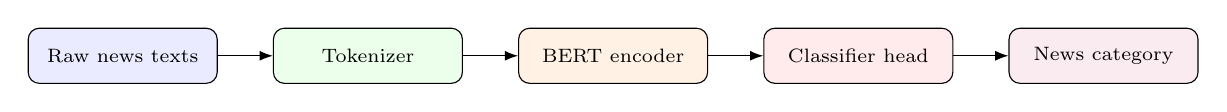
\begin{tikzpicture}[node distance=0.45cm, every node/.style={font=\scriptsize}]
    \node[draw, rounded corners, fill=blue!8, minimum width=2.4cm, minimum height=0.7cm] (raw) {Raw news texts};
    \node[draw, rounded corners, fill=green!8, minimum width=2.4cm, minimum height=0.7cm, right=0.7cm of raw] (tok) {Tokenizer};
    \node[draw, rounded corners, fill=orange!10, minimum width=2.4cm, minimum height=0.7cm, right=0.7cm of tok] (bert) {BERT encoder};
    \node[draw, rounded corners, fill=red!8, minimum width=2.4cm, minimum height=0.7cm, right=0.7cm of bert] (cls) {Classifier head};
    \node[draw, rounded corners, fill=purple!8, minimum width=2.4cm, minimum height=0.7cm, right=0.7cm of cls] (pred) {News category};
    \draw[-{Latex}] (raw) -- (tok);
    \draw[-{Latex}] (tok) -- (bert);
    \draw[-{Latex}] (bert) -- (cls);
    \draw[-{Latex}] (cls) -- (pred);
\end{tikzpicture}
\end{center}

\vspace{0.5cm}

The notebook shows the full pipeline: from raw text to tokenized tensors, from BERT representations to class scores, and from class scores to final predictions.
\end{frame}

%---------------------------------------------------------------------------------------------------
\begin{frame}{Important implementation caveats}
There are some points worth discussing with students.

\begin{itemize}
    \item The notebook uses \texttt{ReLU} after the final linear layer. For \texttt{CrossEntropyLoss}, the usual choice is to return raw logits without a final activation.
    \item The tokenizer example uses \texttt{max\_length=60}, while the full dataset uses \texttt{max\_length=512}. This difference should be explicitly explained.
    \item The batch size is very small, which is convenient for demonstration but inefficient for serious training.
    \item Full fine-tuning of BERT may be slow on CPU and is much more practical on GPU.
\end{itemize}
\end{frame}

%---------------------------------------------------------------------------------------------------
\begin{frame}{Possible improvements for a teaching version}
A more robust teaching notebook could add:
\begin{itemize}
    \item a clearer separation between inference and fine-tuning examples;
    \item explicit train, validation, and test metrics at each epoch;
    \item a confusion matrix and per-class precision, recall, and F1-score;
    \item a comparison between frozen BERT and fully fine-tuned BERT;
    \item reproducible environment specifications for \texttt{torch}, \texttt{transformers}, \texttt{accelerate}, and \texttt{protobuf}.
\end{itemize}
\end{frame}

%---------------------------------------------------------------------------------------------------
\begin{frame}{Key takeaways}
\begin{itemize}
    \item BERT-like models transform text into contextual token representations.
    \item The tokenizer is not a minor detail: it defines the numerical input seen by the model.
    \item For classification, the \texttt{[CLS]} representation is commonly used as a sequence-level feature.
    \item DistilBERT is useful when we need faster and lighter inference.
    \item Fine-tuning adapts a general language model to a specific supervised task.
\end{itemize}
\end{frame}

%---------------------------------------------------------------------------------------------------
\begin{frame}{References mentioned in the notebook}
\begin{itemize}
    \item Hugging Face Transformers documentation.
    \item Hugging Face BERT model documentation.
    \item Ruben Winastwan, \textit{Text Classification with BERT in PyTorch}.
    \item Rayyan Shaikh, \textit{Mastering BERT: A Comprehensive Guide from Beginner to Advanced in Natural Language Processing}.
    \item Jay Alammar, \textit{A Visual Guide to Using BERT for the First Time}.
\end{itemize}
\end{frame}

%===================================================================================================
\end{document}
%===================================================================================================
